\documentclass[10pt]{article}
\usepackage[margin=1in, paperwidth=8.5in, paperheight=11in]{geometry}
\usepackage{ifpdf, amsmath, amssymb, comment, color, graphicx, stmaryrd, setspace, enumitem, fancyhdr, wrapfig, textcomp, mathptmx, siunitx, multicol}
\usepackage{hyperref}
\hypersetup{
    colorlinks=true,
    urlcolor=blue,
}

\usepackage{tikz}
\usetikzlibrary{trees}

\setlength{\headheight}{14.5pt}
\newcommand{\del}{\nabla}
\newcommand{\Q}{\mathbb{Q}}
\newcommand{\R}{\mathbb{R}}
\newcommand{\Z}{\mathbb{Z}}
\newcommand{\vu}{\mathbf{u}}
\newcommand{\vv}{\mathbf{v}}
\newcommand{\vw}{\mathbf{w}}
\newcommand{\vi}{\mathbf{i}}
\newcommand{\vj}{\mathbf{j}}
\newcommand{\vk}{\mathbf{k}}
\newcommand{\vn}{\mathbf{n}}
\newcommand{\vr}{\mathbf{r}}
\newcommand{\vs}{\mathbf{s}}
\newcommand{\va}{\mathbf{a}}
\newcommand{\vF}{\mathbf{F}}
\newcommand{\vL}{\mathbf{L}}
\newcommand{\vT}{\mathbf{T}}
\newcommand{\vN}{\mathbf{N}}
\newcommand{\vB}{\mathbf{B}}
\newcommand{\comp}{\operatorname{comp}}
\newcommand{\proj}{\operatorname{proj}}
\newcommand{\orth}{\operatorname{orth}}
\newcommand\dotp[1][.5]{\,\mathbin{\vcenter{\hbox{\scalebox{#1}{$\bullet$}}}}\,}


\newenvironment{red}{\color{red}}{\ignorespacesafterend}
\newcommand{\blue}[1]{\textcolor{blue}{#1}}
\newcommand{\green}[1]{\textcolor{green}{#1}}
\renewcommand{\section}[1]{\begin{center} \textbf{#1} \\\end{center}}
%
\hyphenpenalty=5000
\setlength{\parindent}{0in}
%\oddsidemargin=-.25in
\allowdisplaybreaks
\pagestyle{fancy}
\renewcommand{\headrulewidth}{0pt}
\lhead{MATH 203}
\rhead{Fall 2024}
%\lfoot{}
%\cfoot{}

\begin{document}
%


%\onehalfspacing
\allowdisplaybreaks
%##################################################################
\section{Checkpoint: Directional derivatives}
The function $T(x,y) = 30 - x^2 - y^2$ measures the temperature, in degrees Celsius, at a given point $(x,y)$ on a heated metal plate, where $x$ and $y$ are measured in centimeters. An ant is walking on this plate in a straight line from the point $(1,2)$ to the point $(4,5)$. Here's a contour plot with some relevant points highlighted.

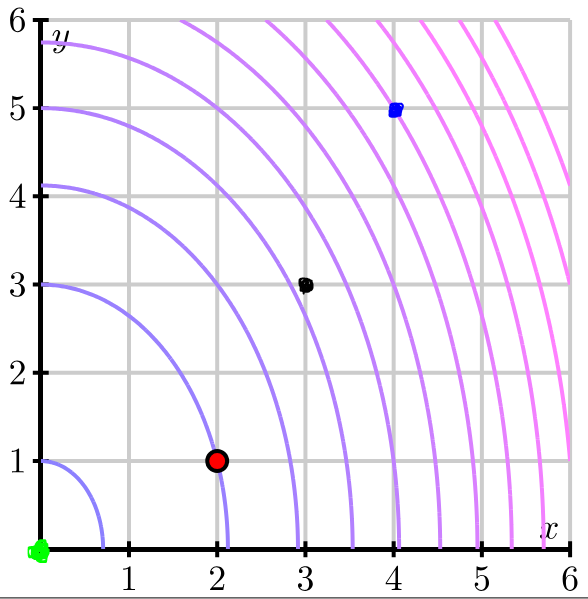
\includegraphics[width=0.6\textwidth]{../images/checkpoint-directional-derivatives.png}

\begin{enumerate}[(a)]
    \item How fast is the temperature under the ant's feet changing at the beginning of its journey? Give units.
    \item How fast is the temperature under the ant's feet changing when it's halfway through its journey? (Hint: if you draw this out you'll see that this is at the point $(3,3)$.)
    \item The ant reaches $(4,5)$ and decides to walk directly back to the origin. Now how fast is the temperature under the ant's feet changing?
\end{enumerate}
	
\end{document}